\apendice{Plan de Proyecto Software}

\section{Introducción}
En este anexo se va a exponer la planificación temporal y el estudio de viabilidad del proyecto.

La planificación temporal está dividida en los \textit{sprints} seguidos para la realización del proyecto.
Cada apartado dentro de la planificación cuenta con información sobre la reunión de planificación del \textit{sprint}, de la que se obtienen conjunto de tareas a realizar, y la reunión de revisión, donde se muestra y valora el trabajo realizado.

\section{Planificación temporal}
Durante este proyecto se ha seguido una metodología Scrum con algunos cambios ya que no se hacían reuniones diarias ni los roles estaban tan marcados, pero la forma de trabajar era la misma con planificaciones y revisiones de \textit{sprints}.
Los \textit{sprints} que se han realizado son los siguientes:

\subsubsection{\textit{Sprint} 1: \textit{Sprint} inicial}
Fechas: 28 febrero 2023 -- 7 marzo 2023.
\begin{itemize}
\item\textbf{Planificación del \textit{sprint}}

En la reunión de planificación del sprint se fijaron las siguientes tareas:
\begin{enumerate}
	\item Configuración inicial del repositorio
	\item Prototipos de las vistas de la aplicación
	\item Creación diagrama entidad-relación
\end{enumerate}

\item\textbf{\textit{Burndown Report}}

\begin{figure}
	\centering
	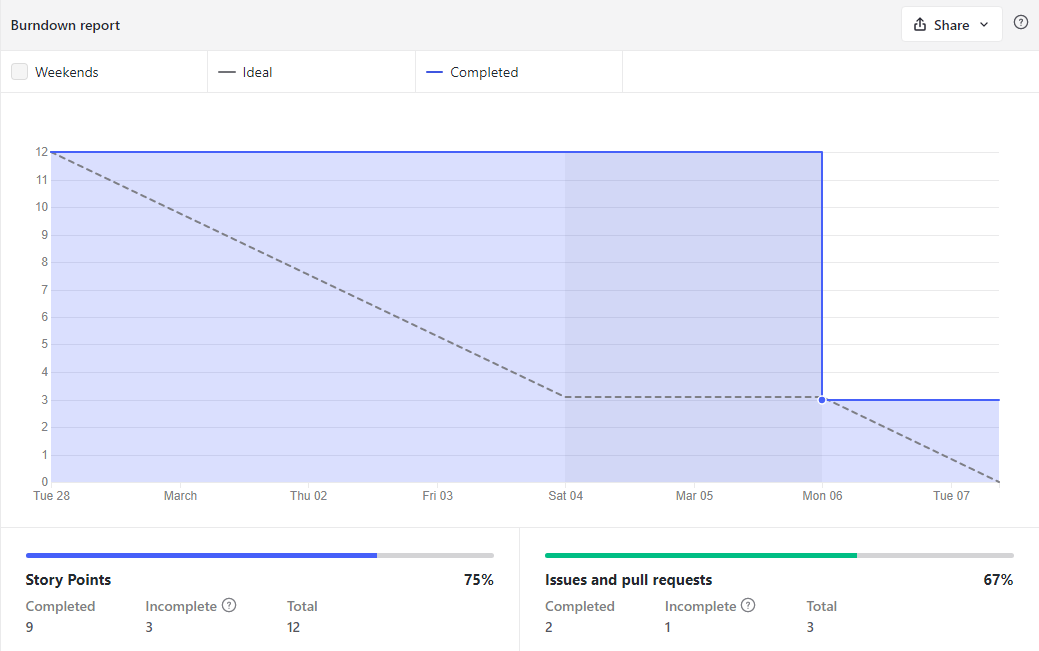
\includegraphics[width=\textwidth]{../img/Anexos/Sprints/Sprint1.png}
	\caption{\textit{Burndown Report Sprint 1}}\label{ReportSprint1}
\end{figure}

Como se puede apreciar en la figura~\ref{ReportSprint1}, no todas las tareas aparecen como completadas. Esto es debido a que el diagrama entidad-relación se dejó abierto ya que faltaba información para completarlo.

\item\textbf{Revisión del \textit{sprint}}

Durante la revisión se mostró el trabajo realizado y se vieron los cambios que se debían realizar en el diagrama entidad-relación que a su vez implicaban cambios en los prototipos de las vistas de la aplicación.
Se llegó a la conclusión de que podía ser buena idea dividir el diagrama E/R haciendo vistas del mismo para que fuere más fácil resolverlo.
\end{itemize}


\subsubsection{\textit{Sprint} 2: Casos de uso y diagrama E/R de cada caso}
Fechas: 7 marzo 2023 -- 14 marzo 2023.
\begin{itemize}
\item\textbf{Planificación del \textit{sprint}}

En la reunión de planificación del sprint se fijaron las siguientes tareas:
\begin{enumerate}
	\item Creación de casos de uso junto a su vista del diagrama E/R.
	\item Aprendizaje de Flask.
\end{enumerate}

\item\textbf{\textit{Burndown Report}}

\begin{figure}
	\centering
	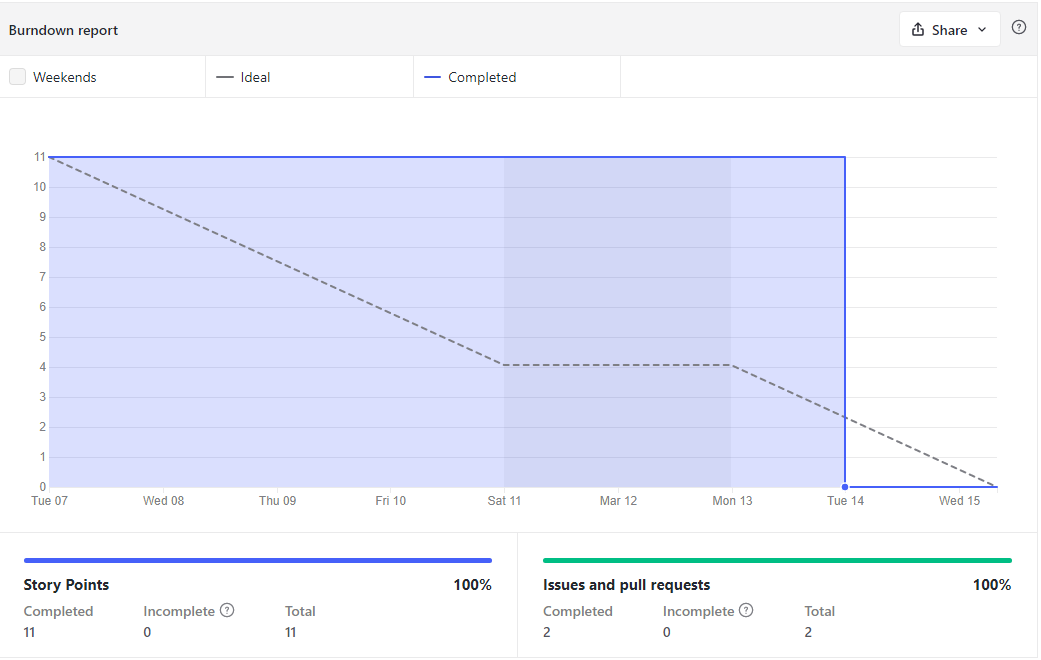
\includegraphics[width=\textwidth]{../img/Anexos/Sprints/Sprint2.png}
	\caption{\textit{Burndown Report Sprint 2}}\label{ReportSprint2}
\end{figure}

En este \textit{sprint} se completaron las tareas marcadas en el tiempo fijado durante la reunión de planificación, pero muchas cosas quedaron pendientes de cambios en futuros \textit{sprints}. En la figura~\ref{ReportSprint2} se puede ver el \textit{Burndown Report} del \textit{sprint}.

\item\textbf{Revisión del \textit{sprint}}

En la reunión de revisión se estudió de nuevo el diagrama E/R y se indicaron nuevos cambios menores en el mismo. También se propuso el comenzar a realizar el diagrama de casos de uso y continuar con el estudio de Flask.
\end{itemize}

\subsubsection{\textit{Sprint} 3: Documentación de casos de uso e investigación y aprendizaje de Flask y bibliotecas JavaScript}
Fechas: 14 marzo 2023 -- 21 marzo 2023.
\begin{itemize}
\item\textbf{Planificación del \textit{sprint}}

En la reunión de planificación del sprint se fijaron las siguientes tareas:
\begin{enumerate}
		\item Realizar el diagrama de casos de uso
		\item Cambios en las vistas adaptándolas a los casos de uso
		\item Documentar los casos de uso con sus tablas
		\item Investigar bibliotecas de JavaScript que pudiesen ayudar
		\item Aprender sobre Flask
\end{enumerate}

\item\textbf{\textit{Burndown Report}}

\begin{figure}
	\centering
	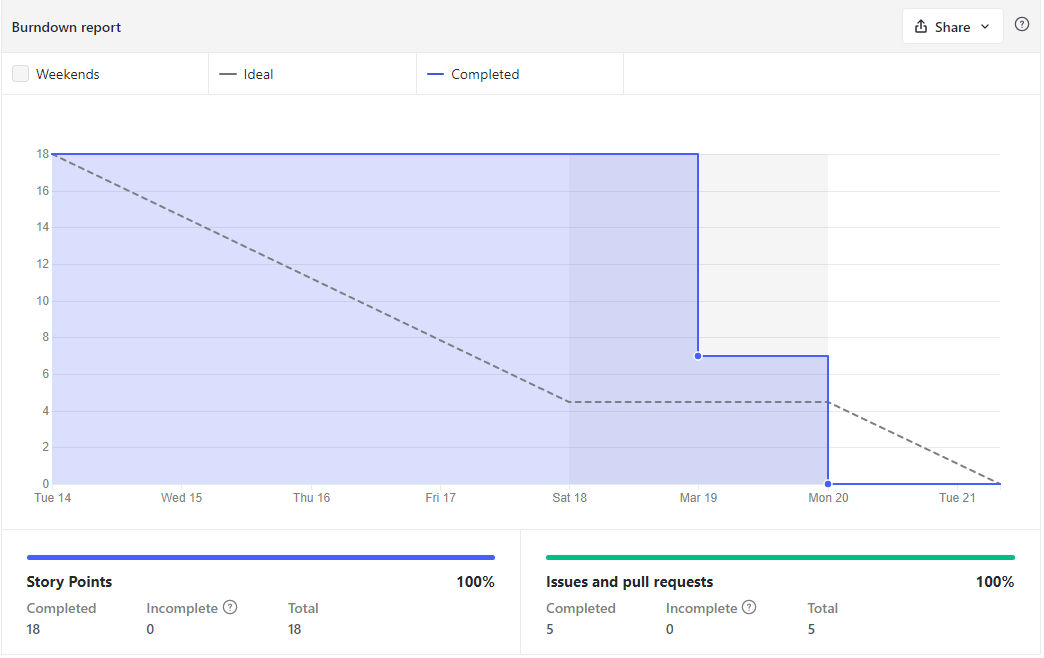
\includegraphics[width=\textwidth]{../img/Anexos/Sprints/Sprint3.png}
	\caption{\textit{Burndown Report Sprint 3}}\label{ReportSprint3}
\end{figure}

En este \textit{sprint} se completaron las tareas marcadas aunque el tiempo marcado para el aprendizaje de Flask fue menor debido a falta de tiempo durante esta semana. Estaba previsto dedicar en total 18 horas al \textit{sprint}, pero finalmente fueron 15. En la figura~\ref{ReportSprint3} se puede ver el \textit{Burndown Report} del \textit{sprint}.

\item\textbf{Revisión del \textit{sprint}}

Durante la revisión se vio que había casos de uso que no eran necesarios y que se podían añadir como excepciones de otros. Esto produjo que el diagrama de casos de uso se debía cambiar, lo que implica un cambio en la documentación de las tablas y en los prototipos de las vistas de la aplicación.
\end{itemize}

\subsubsection{\textit{Sprint} 4: Cambios en los casos de uso y vistas, documentación y Flask}
Fechas: 21 marzo 2023 -- 28 marzo 2023.
\begin{itemize}
\item\textbf{Planificación del \textit{sprint}}

En la reunión de planificación del sprint se fijaron las siguientes tareas:
\begin{enumerate}
		\item Cambios en el diagrama de casos de uso dividiendo en diagrama por niveles y crear vistas del diagrama E/R para los casos de uso.
		\item Cambios en algunos prototipos de las vistas de la aplicación.
		\item Cambios en la documentación de los casos de uso (tablas).
		\item Añadir documentación.
		\item Comenzar estructura básica de la aplicación en Flask.
\end{enumerate}

\item\textbf{\textit{Burndown Report}}

\begin{figure}
	\centering
	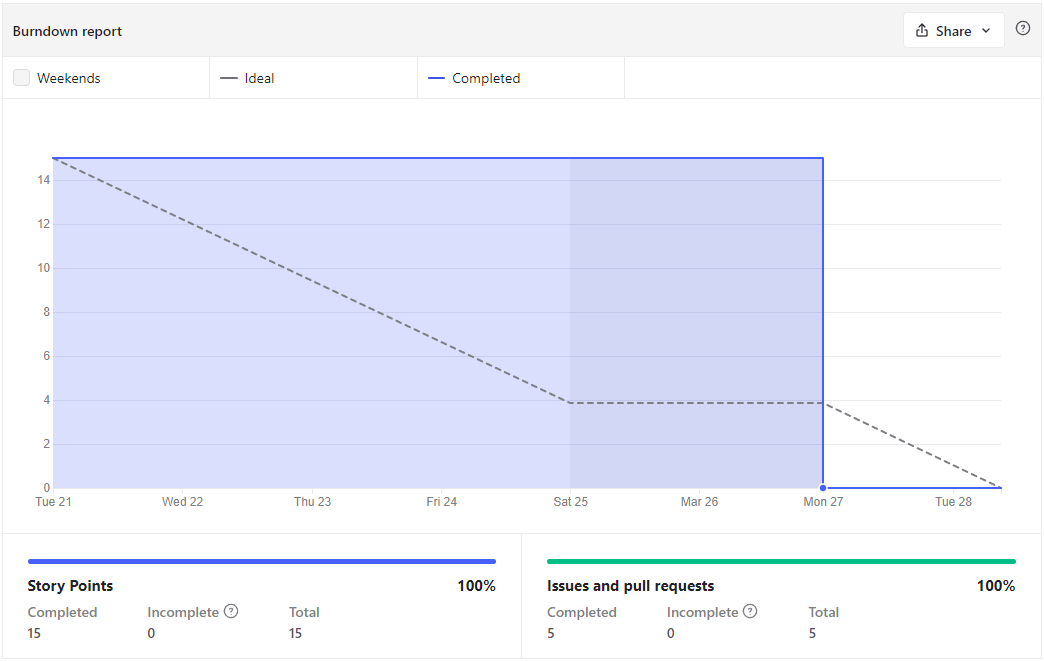
\includegraphics[width=\textwidth]{../img/Anexos/Sprints/Sprint4.png}
	\caption{\textit{Burndown Report Sprint 4}}\label{ReportSprint4}
\end{figure}

A lo largo del \textit{sprint} se realizaron la mayoría de tareas marcadas, pero en las tareas de añadir documentación y comenzar con Flask, no se hizo tanto como estaba esperado debido a la falta de tiempo. 
Se planeo que se iban a poder dedicar más horas de las que al final se dedicaron y no se avanzó todo lo planeado en estas tareas. 
Aún así, se decidió cerrarlas, ya que algo si se había avanzado, y crear de nuevo tareas similares en próximos \textit{sprints}.

La tarea de <<Cambios en el diagrama de casos de uso dividiendo en diagrama por niveles y crear vistas del diagrama E/R para los casos de uso>> tenía una previsión de 2 horas que se realizó en el plazo estimado, la tarea <<Cambios en algunos prototipos de las vistas de la aplicación>> tenía una estimación de 3 horas aunque finalmente fueron 4, la tarea <<Cambios en la documentación de los casos de uso (tablas)>> tenía marcada 4 horas de duración que finalmente fueron 5, la tarea de <<Añadir documentación>> tenía pensada una dedicación de 3 horas que al final se quedó en 1 hora y media aproximadamente y, por último, la tarea <<Comenzar estructura básica de la aplicación en Flask.>> tenía una previsión de 3 horas que quedó reducida a una media hora por falta de tiempo durante el \textit{sprint}. 
En la figura~\ref{ReportSprint4} se puede ver el \textit{Burndown Report} del \textit{sprint}.

\item\textbf{Revisión del \textit{sprint}}

En la reunión de revisión del \textit{sprint} se decidió hacer algunos cambios en los casos de uso, lo que implica un cambio en la documentación de las tablas y los prototipos de las vistas ya que el funcionamiento esperado de la aplicación cambia. También se decidió realizar algún cambio en el diagrama E/R añadiendo nuevos atributos y sacando un atributo a una nueva entidad.
\end{itemize}

\subsubsection{\textit{Sprint} 5: Documentación y comienzo de la aplicación}
Fechas: 28 marzo 2023 -- 11 abril 2023.
\begin{itemize}
\item\textbf{Planificación del \textit{sprint}}

En la reunión de planificación del sprint se fijaron las siguientes tareas:
\begin{enumerate}
		\item Cambios en el diagrama E/R y en algún caso de uso.
		\item Cambios en algunas tablas de los CU y en sus respectivas vistas.
		\item Evaluar plugins/frameworsk para tablas.
		\item Añadir documentación.
		\item Desarrollo de la aplicación.
\end{enumerate}

\item\textbf{\textit{Burndown Report}}

En este \textit{sprint} surgió un problema con herramienta ZenHub que utilizaba para llevar un seguimiento de los \textit{sprints} desde GitHub. Es una herramienta de pago que en teoría cuenta con versiones gratuitas para proyectos \textit{open source} y para profesores. Contacté con ellos para poder obtener una licencia gratuita de la herramienta, pero no fue posible conseguirla. Por lo tanto, a partir de este \textit{sprint} no pude utilizar la herramienta y no pude sacar la imagen del \textit{Burndown Report}.

Para la tarea de <<Cambios en el diagrama E/R y en algún caso de uso>> se estimaba un tiempo de realización de 1 hora que se cumplió.

Para la tarea <<Cambios en algunas tablas de los CU y en sus respectivas vistas>> se puso una estimación de 5 horas que finalmente fueron 7 horas.

Para la tarea <<Evaluar plugins/frameworsk para tablas>> se había marcado una planificación de 2 horas que se cumplió, excediendo un poco de la planificación, ya que aparte de buscar y valorar distintas librerías de JavaScript para la visualización de tablas estuve haciendo pruebas con la librería Grid.js que decidí utilizar para el proyecto.

La tarea de <<Añadir documentación>> tenía marcada una planificación de 3 horas que se cumplió dentro del plazo.

Por último, la tarea de <<Desarrollo de la aplicación>>, donde se buscaba empezar con la aplicación web, tenía una estimación de 8 horas que se convirtió en unas 10 horas de trabajo real debido a algunos problemas surgidos durante el desarrollo.

\item\textbf{Revisión del \textit{sprint}}

En la reunión de revisión se estuvo viendo el trabajo realizado durante el \textit{sprint}. En la parte de documentación se decidió que se debían hacer algunos pequeños cambios en las tablas de los casos de uso, la visualización de imágenes, cambios de orden en un diagrama y cambios en algún título.

En la parte de desarrollo de la aplicación web se decidió realizar algunos cambios en la visualización de tablas para que no ocupasen tanta pantalla así como en el menú de la web para hacerlo más pequeño introduciendo submenús. También se dijo que era mejor poner un selector de centro en la pantalla de la asignación de horas para que de esta forma ya saliesen los datos de la tabla filtrados por centro. 
\end{itemize}

\subsubsection{\textit{Sprint} 6: Base de datos y comenzar a dar funcionalidad a la web}
Fechas: 11 abril 2023 -- 24 abril 2023.
\begin{itemize}
\item\textbf{Planificación del \textit{sprint}}

En la reunión de planificación del sprint se fijaron las siguientes tareas:
\begin{enumerate}
		\item Creación de los modelos y la base de datos en base a los modelos.
		\item Crear la primera carga de la base de datos con CSV y script SQL.
		\item Creación de más vistas junto a su funcionalidad.
		\item Cambios en la documentación.
		\item Añadir más documentación.
\end{enumerate}

\item\textbf{\textit{Burndown Report}}

Este \textit{sprint} tenía una duración inicial de una semana, pero debido a falta de tiempo por exámenes y entregas de trabajos, decidí aplazar una semana más la reunión de revisión para poder trabajar en el proyecto. 
Además, se tuvo que cambiar la fecha habitual de las reuniones debido a que empecé prácticas en una empresa y ya no era compatible la hora/día que se tenía.

La primera tarea completada fue la de <<Creación de los modelos y la base de datos en base a los modelos>>. 
Se puso una estimación de 4 horas, que de trabajo real fue el doble, unas 8 horas. 
Este exceso de tiempo fue debido en gran medida a errores surgidos a la hora de crear la base de datos utilizando el \textit{ORM} SQLAlchemy. 
Los problemas eran principalmente por como hacía la carga de la base de datos que hacía que en algunos contextos estuviese disponible y en otros no, provocando errores al ejecutar la aplicación y generar las tablas de la base de datos.

La tarea <<Crear la primera carga de la base de datos con CSV y script SQL>> tenía una planificación de 2 horas y se completó en el tiempo. 
Sólo quedo pendiente el hecho de que desde la interfaz phpMyAdmin que estoy utilizando para manejar la base de datos, no fui capaz de cargar los archivos csv desde el script de SQL y tuve que cargarlos por separado desde la interfaz.

Para la tarea <<Creación de más vistas junto a su funcionalidad>> se tenía una estimación de 6 horas. 
En este caso fui bastante optimista y el trabajo real termino siendo de 9 horas.
Esto se debido en gran parte a la aparición de problemas que hicieron que tuviera que trabajar más horas de las planeadas en esta tarea.

La tarea <<Cambios en la documentación>> tenía planificadas 2 horas de trabajo. 
En horas reales termino siendo 2 horas y media aproximadamente.

Finalmente, la tarea de <<Añadir más documentación>> tenía una estimación de 1 hora y el trabajo realizado fue también de 1 hora. 
Se añadió sobre todo documentación sobre técnicas y herramientas, apartado de diseño y apartado de plan de proyecto.

\item\textbf{Revisión del \textit{sprint}}

En la reunión de revisión del \textit{sprint} 6 se estuvieron valorando los cambios realizados y las nuevas funcionalidades añadidas.
También se resolvieron algunas dudas sobre la documentación y algunas partes de la funcionalidad de la aplicación web.
Se discutieron algunos aspectos como el añadir algún nuevo campo en la base de datos para códigos internos o cómo tratar la eliminación de los centros, que hasta ahora se trataba como una eliminación en cascada, y se decidió cambiar al existir demasiado riesgo de pérdida de información por un borrado accidental o poco planificado.

\end{itemize}


\subsubsection{\textit{Sprint} 7: Creación de CRUDs y documentar}
Fechas: 24 abril 2023 -- 2 mayo 2023.
\begin{itemize}
\item\textbf{Planificación del \textit{sprint}}


En la reunión de planificación del sprint se fijaron las siguientes tareas:
\begin{enumerate}
		\item Comentarios sobre memoria y anexos.
		\item Crear el CRUD de Docentes, Plazas, Contratos, Áreas y Departamentos.
		\item Solucionar bug con las abreviaturas al modificar una asignatura.
		\item Algunos cambios en campos de la base de datos.
		\item Buscar cómo cargar un CSV desde un script de SQL en phpMyAdmin.
		\item Añadir documentación.
\end{enumerate}

\item\textbf{\textit{Burndown Report}}

La tarea de <<Comentarios sobre memoria y anexos>> fue una tarea creada por Álvar Arnaiz González para dejar las correcciones hechas en la memoria y los anexos. 
Esta tarea fue reutilizada para indicar que se iban a subir esos cambios en la documentación. 
Tenía una planificación de 30 minutos y se realizó dentro del tiempo estimado.

La tarea <<Crear el CRUD de Docentes, Plazas, Contratos, Áreas y Departamentos>> era la que tenía más carga de trabajo en este \textit{sprint} con una estimación de 8 horas que se convirtió en 11 horas de trabajo real.
Este incremento de horas se debió principalmente a problemas para configurar correctamente la biblioteca Select2 utilizando Ajax y para mantener las opciones marcadas en el campo en las modificaciones.

La tarea <<Solucionar bug con las abreviaturas al modificar una asignatura>> era debida a errores en el campo Select2 al hacer una modificación de una asignatura. 
Las abreviaturas de la asignatura aparecían bien, pero no se recuperaban de forma correcta en el servidor para saber cuales habían sido añadidas o eliminadas.
Esta tarea tenía una estimación de 1 hora y no se pretendía superar ese tiempo de trabajo, ya que en la reunión de planificación no se consideró que fuese un problema crucial debido a que en este momento no era necesario que una asignatura tuviera varias abreviaturas y podía ser cambiado por un campo de texto normal que no diese ese problema y permitiese a una asignatura tener una única abreviatura.
Al realizar la tarea anterior se tuvo un problema parecido que dio la pista para resolver este problema dejándolo totalmente subsanado.

La tarea <<Algunos cambios en campos de la base de datos>> tenía una estimación de 1 hora y se realizó dentro del plazo.
La tarea consistía en añadir nuevos campos en la base de datos, lo que suponía también hacer cambios en el código para introducir los nuevos atributos en los modelos y en los formularios.
También se cambió el borrado en cascada que tenían los centros para evitar que se eliminen centros que tengan titulaciones vinculadas.

Para la tarea <<Añadir documentación>> se estimaron 3 horas de trabajo que se cumplieron en cuanto a trabajo real.

Finalmente, para la tarea <<Buscar cómo cargar un CSV desde un script de SQL en phpMyAdmin>> se estimó 1 hora de trabajo que finalmente fue un trabajo real de 2 horas debido a que tuve que investigar por los problemas que me daba con la carga de los ficheros csv. El problema finalmente fue donde estaban colocados los csv.


\item\textbf{Revisión del \textit{sprint}}

En la reunión de revisión se mostró el trabajo realizado y se resolvieron algunas dudas acerca de la memoria y algunas partes del funcionamiento de la aplicación web.
\end{itemize}


\subsubsection{\textit{Sprint} 8: Gestión de cursos}
Fechas: 2 mayo 2023 -- 15 mayo 2023.
\begin{itemize}
\item\textbf{Planificación del \textit{sprint}}


En la reunión de planificación del sprint se fijaron las siguientes tareas:
\begin{enumerate}
		\item Subir la web a Heroku.
		\item Programar el apartado ge gestión de cursos.
		\item Hacer pequeños cambios en la web.
		\item Añadir documentación de trabajos relacionados.
\end{enumerate}

\item\textbf{\textit{Burndown Report}}

La primera tarea que se realizó fue <<Subir la web a Heroku>>.
La tarea tenía una carga de trabajo estimada en 2 horas.
Para esta tarea la estimación no fue nada correcta, ya que el trabajo real fue aproximadamente de 8 horas.
Esto fue debido principalmente a problemas a la hora de configurar el proyecto para ser reconocido por la plataforma Heroku y para configurar correctamente la base de datos. 
Surgieron un gran listado de problemas que fueron resueltos uno por uno hasta que la instalación fue satisfactoria.

Para la tarea <<Programar el apartado ge gestión de cursos>> se habían marcado 8 horas de trabajo que finalmente se convirtieron en mucho más, 20 horas de trabajo.
Esta gran discrepancia entre la planificación y el trabajo real fue debida en gran medida a la investigación y planteamiento de cómo mostrar el listado de asignaturas que se deben seleccionar a la hora de crear un curso.
Se intentó crear de la forma más cómoda para utilizar y con el menor impacto posible en el rendimiento.
También surgieron algunos problemas durante la programación que fueron subsanados pero que hicieron que el tiempo de trabajo se fuese desplazando aun más de la estimación realizada.

La siguiente tarea fue <<Hacer pequeños cambios en la web>>.
Esta tarea tenía una estimación de 3 horas que de trabajo real en realidad fueron unas 2 horas. 
Estos pequeños cambios eran principalmente sobre la visualización del contenido.

Finalmente, la tarea <<Añadir documentación de trabajos relacionados>> tenía una estimación de trabajo de 1 hora y el trabajo real tuvo también una duración aproximada de una hora.


\item\textbf{Revisión del \textit{sprint}}

Durante la reunión de revisión se vieron principalmente los cambios realizados en la web. Se estuvieron discutiendo diferentes formas de crear los cursos y se llegó a la conclusión de hacer pequeños cambios para que fuese más cómoda la creación de cursos.
También se estuvieron viendo las diferentes secciones de la memoria para dar ideas sobre la documentación que se podía ir introduciendo.
\end{itemize}


\subsubsection{\textit{Sprint} 9: Cambios, gestión de grupos y documentación}
Fechas: 15 mayo 2023 -- 23 mayo 2023.
\begin{itemize}
\item\textbf{Planificación del \textit{sprint}}


En la reunión de planificación del sprint se fijaron las siguientes tareas:
\begin{enumerate}
		\item Algunos cambios en la gestión de cursos.
		\item Creación de la gestión de grupos.
		\item Pequeños cambios/mejoras en el código.
		\item Avanzar en la memoria.
\end{enumerate}

\item\textbf{\textit{Burndown Report}}

Para la tarea <<Algunos cambios en la gestión de cursos>> se fijaron 4 horas. 
Esta tarea tenía como propósito realizar los cambios vistos en la reunión de revisión del \textit{sprint} anterior.
Estos cambios llevaron unas 3 horas de trabajo, pero debido a algunos errores al realizar los cambios se consumieron las 4 horas planificadas.

La segunda tarea realizada fue <<Creación de la gestión de grupos>>.
En esta tarea se quería crear todo lo relacionado con la gestión de grupos.
Desde su visualización en una tabla, a la creación y eliminación de los mismos para cada asignatura de un curso académico.
Para esta tarea se dio una estimación de 8 horas que en trabajo real fueron algo menos, pero cercano a las 8 horas.

La tercera tarea de <<Pequeños cambios/mejoras en el código>> tenía una estimación de tiempo de 1 hora y se cumplió en este tiempo.
En esta tarea se realizaron algunos cambios menores de diseño, cambios en vistas, algunos pequeños cambios de lógica, etc.

Finalmente, la tarea de <<Avanzar en la memoria>> tenía una estimación de 3 horas.
En esta tarea se pretendían realizar los cambios vistos en la documentación y añadir nueva información a la memoria.
La tarea llevó un trabajo real de aproximadamente las 3 horas. Se hicieron avances en la memoria y se añadió en los anexos el diccionario de datos, además de realizar los cambios vistos por toda la documentación.

\item\textbf{Revisión del \textit{sprint}}

En la reunión del \textit{sprint} 9 se estuvieron viendo los avances realizados. Se comentó que podría ser buena idea realizar algunos cambios en la creación de grupos y añadir una vista donde visualizar las titulaciones de un centro y las asignaturas de una titulación. Además, se descubrió un error en la eliminación de grupos y se estuvo hablando sobre como realizar el inicio de sesión de la aplicación a través de un \textit{token} devuelto por la UBU.
\end{itemize}

\subsubsection{\textit{Sprint} 10: Asignación de horas}
Fechas: 23 mayo 2023 -- 29 mayo 2023.
\begin{itemize}
\item\textbf{Planificación del \textit{sprint}}

En la reunión de planificación del sprint se fijaron las siguientes tareas:
\begin{enumerate}
		\item Crear la asignación de horas de plazas a grupos.
		\item Añadir forma avanzada de creación de grupos.
		\item Arreglar la eliminación de grupos.
		\item Cambios de campos obligatorios en "Añadir Plaza".
		\item Arreglo \textit{bug} de números negativos.
		\item Mejoras de navegación en la web.
		\item Añadir documentación en los anexos.
\end{enumerate}

\item\textbf{\textit{Burndown Report}}

Para la tarea <<Crear la asignación de horas de plazas a grupos>> se fijaron 8 horas de trabajo.
La realidad fue un trabajo de aproximadamente 12 horas.
Este exceso de horas es debido a algunas complicaciones para realizar lo deseado que no se habían tenido en cuenta, pero que se fueron solucionando durante el desarrollo.

Para la tarea <<Añadir forma avanzada de creación de grupos>> se realizó una estimación de 4 horas.
Sin embargo, se dejó la tarea pausada hasta la próxima reunión debido a algunas incompatibilidades con el funcionamiento actual del sistema.
En la próxima reunión habrá que decidir si añadir esa funcionalidad cambiando las actuales o descartar la idea.

En la tarea <<Arreglar la eliminación de grupos>> se pretendía arreglar la reasignación de nombres de grupos al eliminar un grupo teórico.
En la creación de esta funcionalidad no se había probado bien y si se eliminaba un grupo teórico al que le pertenecían grupos prácticos, estos no se renombraban y daban lugar a futuros problemas.
Para la realización de la tarea se hizo una estimación de 2 horas y se realizó dentro de ese tiempo.

La tarea <<Cambios de campos obligatorios en "Añadir Plaza">> fue añadida por los tutores del proyecto al probar la aplicación y decidir realizar algunos cambios en los campos que debían ser obligatorios al crear una nueva plaza. 
Tenía una previsión de 15 minutos, pero estos pequeños cambios llevaron entre 20 y 30 minutos debido a que hubo que realizar cambios en la base de datos y, para ello, instalar y configurar una biblioteca para migraciones de la base de datos.

La tarea <<Arreglo \textit{bug} de números negativos>> también fue añadida por los tutores del proyecto al realizar sus pruebas en la web.
Algunos campos no se validaban bien y permitían ingresar números negativos en sitios donde esto no debía se posible.
Estos pequeños cambios llevaron aproximadamente 15 minutos.

La tarea <<Mejoras de navegación en la web>> fue otra de las añadidas por los tutores del proyecto.
Se pretendía mejorar la navegación por la web añadiendo botones de volver atrás sin realizar cambios en los formularios.
Además, se deseaba añadir una ventana desde donde ver las titulaciones de un centro y las asignaturas de una titulación.
Estos cambios tuvieron una estimación de poco más de una hora y, al final, el trabajo real también fue acorde.

Finalmente, para la tarea de <<Añadir documentación en los anexos>> se realizó una estimación de 3 horas.
Debido a falta de tiempo apenas se pudo avanzar y el trabajo real se quedó en aproximadamente media hora.


\item\textbf{Revisión del \textit{sprint}}

En la reunión del \textit{sprint} 10 se estuvieron viendo todos los cambios realizados.
En cuanto a la asignación de horas a plazas se dio el visto bueno, pero se propusieron algunos cambios en la visualización de los datos y se estudió la posibilidad de actualizar alguna información de la tabla mediante \textit{Ajax} al realizar una actualización sobre la misma.

Otro de los aspectos que fueron claves en la reunión fue la creación de grupos de forma avanzada indicando el nombre del grupo. Se llegó a la conclusión de que es una característica que podría ser interesante en un futuro aunque no primordial.
Además, de la forma que se había hecho el diseño era difícil adaptarlo y se decidió dejarlo como una característica interesante para próximas versiones de la aplicación.
\end{itemize}

\subsubsection{\textit{Sprint} 11: Pequeños cambios y arreglos}
Fechas: 29 mayo 2023 -- 5 junio 2023.
\begin{itemize}
\item\textbf{Planificación del \textit{sprint}}

En la reunión de planificación del sprint se fijaron las siguientes tareas:
\begin{enumerate}
		\item Arreglo de \textit{bug} de curso duplicado.
		\item Algunos cambios en la visualización de las horas de plazas en grupos.
		\item Crear el duplicado de la asignación de horas a grupos al duplicar el curso.
		\item Arreglo de \textit{bug} de dos plazas con el mismo docente.
		\item Creación de \textit{login}.
\end{enumerate}

\item\textbf{\textit{Burndown Report}}

Para la tarea <<Arreglo de \textit{bug} de curso duplicado>> se fijaron 30 minutos de trabajo.
La realidad fue un trabajo de aproximadamente el mismo tiempo.
Fue un trabajo sencillo ya que principalmente se basa en comprobar si ya existía un curso con ese año y no permitir crear otro con el mismo año.

La tarea <<Algunos cambios en la visualización de las horas de plazas en grupos>> tenía una estimación de 4 horas.
En esta tarea se pretendía realizar varios cambios en la tabla general de horas sobre como se mostraba la información de los docentes y también cambios dentro de la propia ventana de las plazas asignadas a una asignatura.
El trabajo real fue de 2 horas ya que llevó menos trabajo del pensado en un inicio.

En cuanto a la tarea de <<Crear el duplicado de la asignación de horas a grupos al duplicar el curso>> se puso una estimación de 2 horas.
En esta tarea se pretendía implementar en el duplicado de un curso académico la opción de duplicar también las asignaciones de horas de plazas a las asignaturas del curso.
La tarea llevó aproximadamente las 2 horas estimadas para su realización.

La tarea <<Arreglo de \textit{bug} de dos plazas con el mismo docente>> se estimó en una duración de media hora ya que tan solo era arreglar un pequeño fallo de funcionamiento en el que a un docente se le podía asignar más de una plaza sin que la plaza tuviese fecha de cese.
La idea del funcionamiento es que un docente pueda tener como máximo una plaza sin fecha de cese, es decir, una plaza activa al mismo tiempo.
La duración real fue de poco más de la media hora marcada inicialmente.

Por último, para la tarea <<Creación de \textit{login}>> se puso una estimación de 3 horas.
En esta tarea se implementó el \textit{login} de la aplicación, utilizando para ello el inicio de sesión contra el Moodle de la UBU, el cual devuelve un \textit{token} en caso de inicio de sesión correcto.
Para el inicio de sesión primero se debe verificar que el usuario exista en esta aplicación, si no, por mucho que exista en Moodle, no dejará entrar a la aplicación web.
Además de la creación del \textit{login} se tuvo que implementar la gestión de permisos en todas las acciones de la web para verificar si el usuario estaba identificado o no, y de esta forma dejarle manejar la web o redirigir a la ventana de inicio de sesión.

\item\textbf{Revisión del \textit{sprint}}

En la reunión del \textit{sprint} 11 se dio el visto bueno a los cambios realizados, pero se estuvieron viendo algunos cambios que podrían mejorar la visualización de las horas asignadas a plazas.

También se explicó cómo debían funcionar los permisos en la aplicación web diferenciando de usuarios con permisos de modificación o permisos de lectura. Además de la posibilidad de tener usuarios sin ningún tipo de permiso, caso que se dará cuando se de un docente de baja.

También se vieron diferentes mejoras que se podrían añadir si daba tiempo como un botón para exportar e importar la información de la base de datos, la creación de gráficos con los datos de las horas de asignaturas, etc.
\end{itemize}


\subsubsection{\textit{Sprint} 12: Últimos cambios aplicación}
Fechas: 5 junio 2023 -- 12 junio 2023.
\begin{itemize}
\item\textbf{Planificación del \textit{sprint}}

En la reunión de planificación del sprint se fijaron las siguientes tareas:
\begin{enumerate}
		\item Cambios en el login y creación de campos de lectura y escritura en docente.
		\item Cambios visuales en el apartado de horas.
		\item Creación de opción para importar y exportar la base de datos.
		\item Arreglo de \textit{bug} con los permisos de usuario.
		\item Pequeños cambios de funcionamiento general.
		\item Avanzar documentación.
\end{enumerate}

\item\textbf{\textit{Burndown Report}}

La tarea <<Cambios en el login y creación de campos de lectura y escritura en docente>> tenía una estimación de 3 horas.
En esta tarea lo que se quería hacer era la forma de hacer el \textit{login} y, además, añadir dos campos en la tabla docente para identificar si se tienen permisos de lectura, modificación o ambos, y así mostrar diferentes elementos o vistas según los permisos.
Este trabajo llevó finalmente 5 horas, algo más de lo previsto debido a algunos problemas con la forma de implementar los permisos que se vio que no era le mejor forma y se decidió cambiar de nuevo por una forma más eficiente.
Además, inicialmente se guardaban el \textit{token} y el id del docente en el lado del cliente, cosa que carece en gran medida de seguridad, ya que "robar" una \textit{cookie} es algo relativamente sencillo y esto podría provocar el acceso a la aplicación por usuarios no deseados.
Para solucionar esto, se hizo un cambio para almacenar los datos de la sesión en la base de datos. 
Además, los datos se guardan cifrados, lo que añade muchas más seguridad de esta información sensible.

Para la tarea de <<Cambios visuales en el apartado de horas>> se dió una estimación de 1 hora y el trabajo se realizó en ese tiempo.

En cuanto a la tarea <<Creación de opción para importar y exportar la base de datos>> fue una de las más complejas.
La estimación inicial fue de 3 horas ya que se pensó que iba a ser una tarea relativamente sencilla.
La tarea pretendía añadir una nueva funcionalidad a la web en la que se permite exportar el contenido de la base de datos e importar el contenido descargado previamente.
Esta funcionalidad es interesante pensando en la importación sencilla de los datos cuando se cree una nueva implantación de la web. 

En un principió se pensó que sería una tarea sencilla, pero a la hora de la verdad fue una tarea complicada ya que la conexión y lectura de la base de datos no era algo tan sencillo.
Había que controlar los diferentes tipos de datos y solventar algunos errores con la tabla de sesiones que contaba con información en binario y que se pensó que lo mejor era no exportar esa información ya que no es relevante.

De cara a la importación también llevó mucho tiempo debido a estudiar los diferentes ataques que se podían producir con esta funcionalidad, tanto en la subida del archivo a la web, como en las sentencias incluidas en el SQL.
Finalmente se decidió permitir únicamente las sentencias \textit{insert}, ya que la idea de la funcionalidad es únicamente añadir datos a la base de datos, y así evitar borrados o modificaciones no deseadas.

El trabajo final fue de unas 8 horas, bastante más de lo estimado.

Para la tarea <<Arreglo de \textit{bug} con los permisos de usuario>> se dio una estimación de 20 minutos ya que lo único que se quería hacer era limitar las capacidades de un usuario sin permisos dentro de la aplicación, prohibiéndoles el acceso incluso a la ventana principal.
Actualmente, un usuario sin permisos no puede pasar del inicio de sesión, donde se muestra un mensaje indicando la falta de permisos.

La tarea <<Pequeños cambios de funcionamiento general>> tenía una estimación de 1 hora.
Esta tarea estaba diseñada para realizar algunos cambios visuales o de funcionalidad en la web. Así como carga interna de bibliotecas o datos.
La duración real de la tarea también fue de 1 hora aproximadamente.

Por último, la tarea de <<Avanzar documentación>> tenía una estimación de 4 horas de trabajo que al final se convirtió en...................

\item\textbf{Revisión del \textit{sprint}}

En la reunión del \textit{sprint} 12
\end{itemize}


\section{Estudio de viabilidad}

\subsection{Viabilidad económica}

\subsection{Viabilidad legal}


